\glsresetall
\chapter{Possible Solution}
\label{chap:possible_solution}

In this chapter we present and discuss the possible solution to be implemented regarding the research objectives of this work. To present the solution and explain it, we will cover some aspects and topics that are considered when defining a software based solution. This topics are the well known functional requirements \ref{sec:functional_requirements}, the quality attributes or non-functional requirements \ref{sec:quality_attributes} and finally, the architecture \ref{sec:architecture} that is produced based on all the previous topics.

\begin{figure}[H]
    \centering
    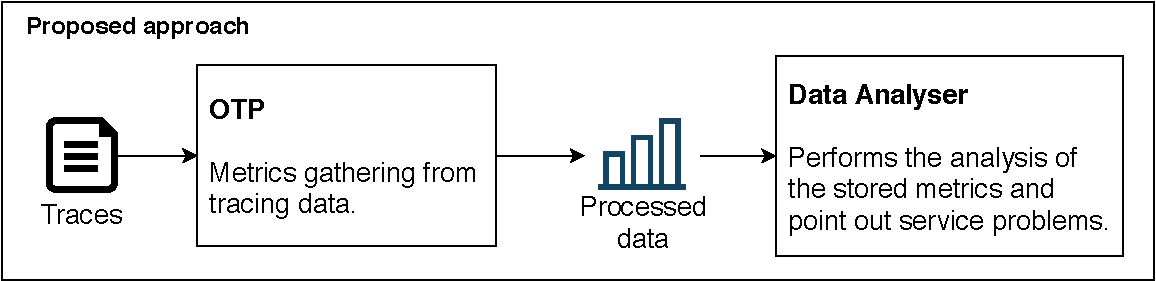
\includegraphics[width=1.00\textwidth]{images/proposed_solution.pdf}
    \caption{Proposed approach for tracing analysis.}
    \label{fig:proposed_approach_for_tracing_analysis}
\end{figure}

% Functional Requirements ------------------------------------------------------------------------
\section{Functional Requirements}
\label{sec:functional_requirements}

The functional requirements are in software and systems engineering, by definition, a declaration of the intended function of a system and its components. For the purpose of this specification, we decided to present a brief description of each functional requirement, composed by an id, the corresponding name and its priority. The notation used in the priority was based on the urgency that we have to implement a certain functionality, and we decided to use three levels: High, Medium and Low priorities.

Therefore, the functional requirements for the proposed solution, obtained from the questions presented in the chapter \ref{chap:research_objectives_and_approach}, are briefly specified in the table \ref{table:functional_requirements_specification} sorted by priority levels.

\begin{table}[!ht]
\caption{Functional requirements specification.}
\label{table:functional_requirements_specification}
\begin{tabularx}{\linewidth} {
    |>{\hsize=0.4\hsize}X| 
     >{\hsize=2.2\hsize}X|
     >{\hsize=0.4\hsize}X| }
    \hline
    \textbf{ID} 
    & \textbf{Name}
    & \textbf{Priority} \\ \hline
    FR-1
    & The system must know what are the neighbours of a certain service, based on the service incoming requests.
    & High \\ \hline
    FR-2
    & The system must know what are the neighbours of a certain service, based on the service outgoing requests.
    & High \\ \hline
    FR-3
    & The system must know which endpoints are the most popular.
    & High \\ \hline
    FR-4
    & The system must know if requests to a certain endpoint results in success or error.
    & High \\ \hline
    FR-5
    & The system must be able to identify if there is any problem related to the response time.
    & Medium \\ \hline
    FR-6
    & The system must be able to identify if there is any problem related to its morphology.
    & Medium \\ \hline
    FR-7
    & The system must be able to identify if there is any problem related to the entire work-flow of one or more requests.
    & Medium \\ \hline
    FR-8
    & The system must know how endpoints orders distributions are done when using a specific endpoint.
    & Medium \\ \hline
    FR-9
    & The system must be able to identify if there is any problem related to the occupation/load.
    & Low \\ \hline
    FR-10
    & The system must be able to identify if there is any problem related to the number/profile of the client requests.
    & Low \\ \hline
\end{tabularx}
\end{table}

As the table \ref{table:functional_requirements_specification} shows us, the functional requirements can be grouped in three main groups due to their priority levels. The first four (FR-1 to FR-4) are presented with high level of priority, because they do not represent a very high level of difficulty to implement, however they provide some base to the implementation of the following four. This four functional requirements (FR-5 to FR-8) represent a much higher degree of difficulty has there are much more questions to solve involving research and the implementation (explained in the chapter \ref{chap:research_objectives_and_approach} - \nameref{chap:research_objectives_and_approach}). The final two (FR-9 and FR-10) have a low priority level, because they do not represent to much relevance of functionality to our core issues.


% Quality Attributes -----------------------------------------------------------------------------
\section{Quality Attributes}
\label{sec:quality_attributes}

When designing a system, one of the most important things to consider is to specify and describe well all the quality attributes or non-functional requirements. These kind of requirements are usually Architecturally Significant Requirements and they are the ones that require more of the architect's attention, as they reflect directly all the architecture decisions and aspects. Sometimes, they are also named the ``itilities'' because most of them share this suffix in the word.

To specify them, we usually use a representation called a utility tree, in which we insert the \gls{qa} by a certain order of priority, for the architecture and for the business inherent to each one, and in order to consider the trade-offs and decide the weight of each in the produced architecture. The codification of the order of priority is the following:

\begin{itemize}
    \item H. High
    \item M. Medium
    \item L. Low
\end{itemize}

To describe them, we must pay attention and try to include six important things in the definition: the \textbf{stimulus source}, the \textbf{stimulus}, the \textbf{environment}, the \textbf{artifact}, the \textbf{response} and the \textbf{measure of the response}.

The figure \ref{fig:utility_tree} contains all the raised \gls{qa} for this project exposed in a utility tree format, sorted alphabetically by their general \gls{qa}, and after by the architectural impact.

\begin{figure}[!ht]
    \centering
    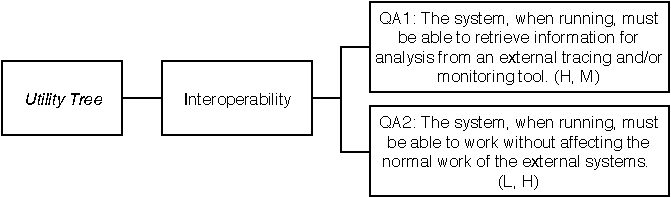
\includegraphics[width=1.00\textwidth]{images/utility_tree.pdf}
    \caption{Utility tree.}
    \label{fig:utility_tree}
\end{figure}

As we can see by the information presented in the utility tree, there are the following \gls{qa}'s: Interoperability, Performance, Scalability, Traceability and Testability. A briefly explanation for every \gls{qa} is exposed bellow:

\begin{itemize}
    \item[\textbf{QA1}] (Interoperability): Since the wanted solution is a monitoring tool, it has to access an external system in order to obtain the necessary data to analyse and therefore, access to an internal monitoring tool presented in the external system. As this is considered the starting point to obtain our data, we considered a Medium level for the architecture and a Low for the business.

    \item[\textbf{QA2}] (Interoperability): Since the solution will be accessing an external system or outputs generated by it, all interactions with it must not cause conflicts. This is very important in the business perspective, because if our solution is not co habitable with other systems it may be completely rejected. For the architectural perspective it doesn't represent a big impact. 
    
    \item[\textbf{QA3}] (Performance): We defined this \gls{qa} taking into account the number of spans produced in an hour, by the system were we gathered our data. As it produces approximately 200.000 spans in an hour, and to ease our research work when using the tool, we decided to set the target for our solution as 1.000.000 spans in about a minute. This \gls{qa} will have an high architectural impact, as it can define a certain technology for graph processing. For the business perspective, we considered a Medium level, as it presents some interest.
    
    \item[\textbf{QA4}] (Scalability): Due to the amount of data needed to process and store over time, our system has to be able to store the data into multiple machines because it may start running out of space. We decided to give a medium level of architectural impact as it can change the solution in terms of storage components. For the business this has an high impact, as it need more machines to run the solution if this \gls{qa} is fully considered against the remaining.
    
    \item[\textbf{QA5}] (Traceability): This \gls{qa} was considered due to the simple fact that we need to bee able to see what's the system is doing, when it's processing the data. For this \gls{qa} we decided to give low levels for both architecture and business, as it does not represent relevance to any of them.
    
    \item[\textbf{QA6}] (Testability): As the system will be analysing external systems, we need to be sure that it analyses it in a correct way, and to be sure of this we need to test our solution. We considered a medium level for the architectural impact for this \gls{qa}, because its implementation needs to analyse some components from within the system. For the business we considered a low level, because the main interest to test the system is ours in order check if it is working correctly.
\end{itemize}


% Technical Restrictions -------------------------------------------------------------------------
\section{Technical Restrictions}
\label{sec:technical_restrictions}

In this section we present the technical restrictions involved in this solution.

Normally, when specifying a solution in software engineering, after presenting the functional requirements and non-functional requirements, comes the specification of business restrictions. However, in this project none were raised due to the simple fact that this work is focused on the exploration and research and that there isn't any formal client defined. 

To define the technical restrictions, we used an id and its corresponding description. The raised technical restrictions are presented in the table \ref{table:technical_restrictions_specification} followed by an explanation.

\begin{table}[!ht]
\caption{Technical restrictions specification.}
\label{table:technical_restrictions_specification}
\begin{tabularx}{\linewidth} {
    |>{\hsize=0.4\hsize}X| 
     >{\hsize=1.6\hsize}X| }
    \hline
    \textbf{ID} 
    & \textbf{Description} \\ \hline
    TR-1
    & Use OpenTSDB as a Time-Series database. \\ \hline
\end{tabularx}
\end{table}

We raise only one technical restriction, as we can see in the table \ref{table:technical_restrictions_specification}. This technical restriction was considered because prof. Jorge Cardoso suggested it, due to the simple fact that OpenTSDB is the database that they are currently using in their projects where a time-series database is needed. However, this project does not have a concrete and formally defined client, it is good to use a technology used by the people that will use the tool to ease their work and possibly introduce changes.


% Architecture -----------------------------------------------------------------------------------
\section{Architecture}
\label{sec:architecture}

In this section, the architecture will be presented based on all the previous topics with resource to the defined Simon Brown’s C4 Model\cite{simon_browns_c4_model}. This approach of defining an architecture uses the following four diagrams to do it: 1 - Context Diagram, 2 - Container Diagram, 3 - Component Diagram and 4 - Code Diagram. For the definition of this architecture, only the first three representations will be considered. Every representation will be exposed with a briefly explanation of the decisions taken to draw that specific diagram. After presenting the representations and the corresponding explanations, we will cycle thought all the \gls{qa}, in order to explain where it is reflected and the considerations taken to produce the current architecture.


% Context Diagram --------------------------------------------------------------------------------
\subsection{Context Diagram}
\label{subsec:context_diagram}

In this subsection the context diagram is presented. This kind of diagram allows us to see ``the big picture'' of the system as it represents the system as a ``big box'' and its interactions with the users and other systems. The figure \ref{fig:context_diagram} presents the context diagram for this solution.

\begin{figure}[!ht]
    \centering
    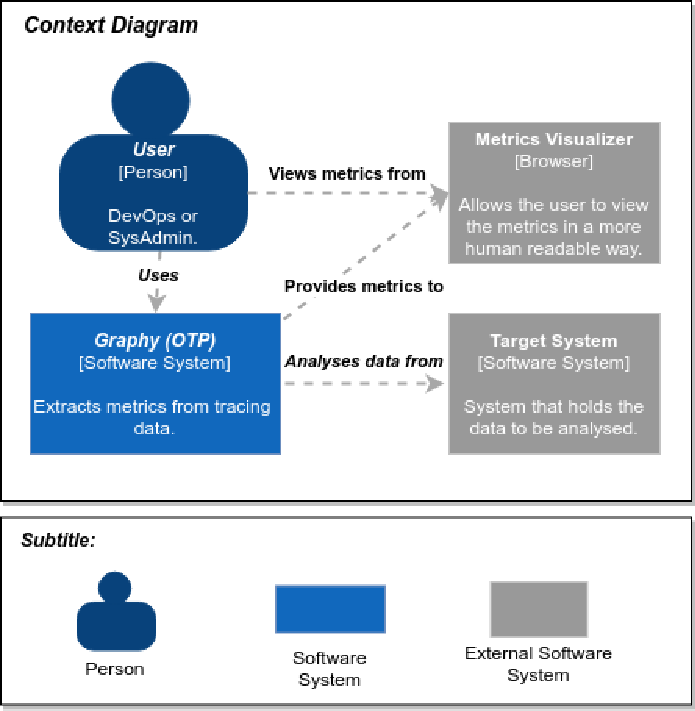
\includegraphics[width=0.75\textwidth]{images/context_diagram.pdf}
    \caption{Context diagram.}
    \label{fig:context_diagram}
\end{figure}

In the presented diagram we can see that the solution, \textit{Graphy}, will receive interactions from the user, as it need someone to control its operations and will analyse data from an external system infrastructure, defined as the target system.


% Container Diagram ------------------------------------------------------------------------------
\subsection{Container Diagram}
\label{subsec:container_diagram}

In this subsection the container diagram is presented. This kind of diagram allows us to perform a ``zoom-in'' in the context diagram, and get a new overview of this system, therefore in this diagram we can see the high-level shape of the software architecture and how responsibilities are distributed across it. The figure \ref{fig:container_diagram} presents the container diagram for this solution.

\begin{figure}[!hb]
    \centering
    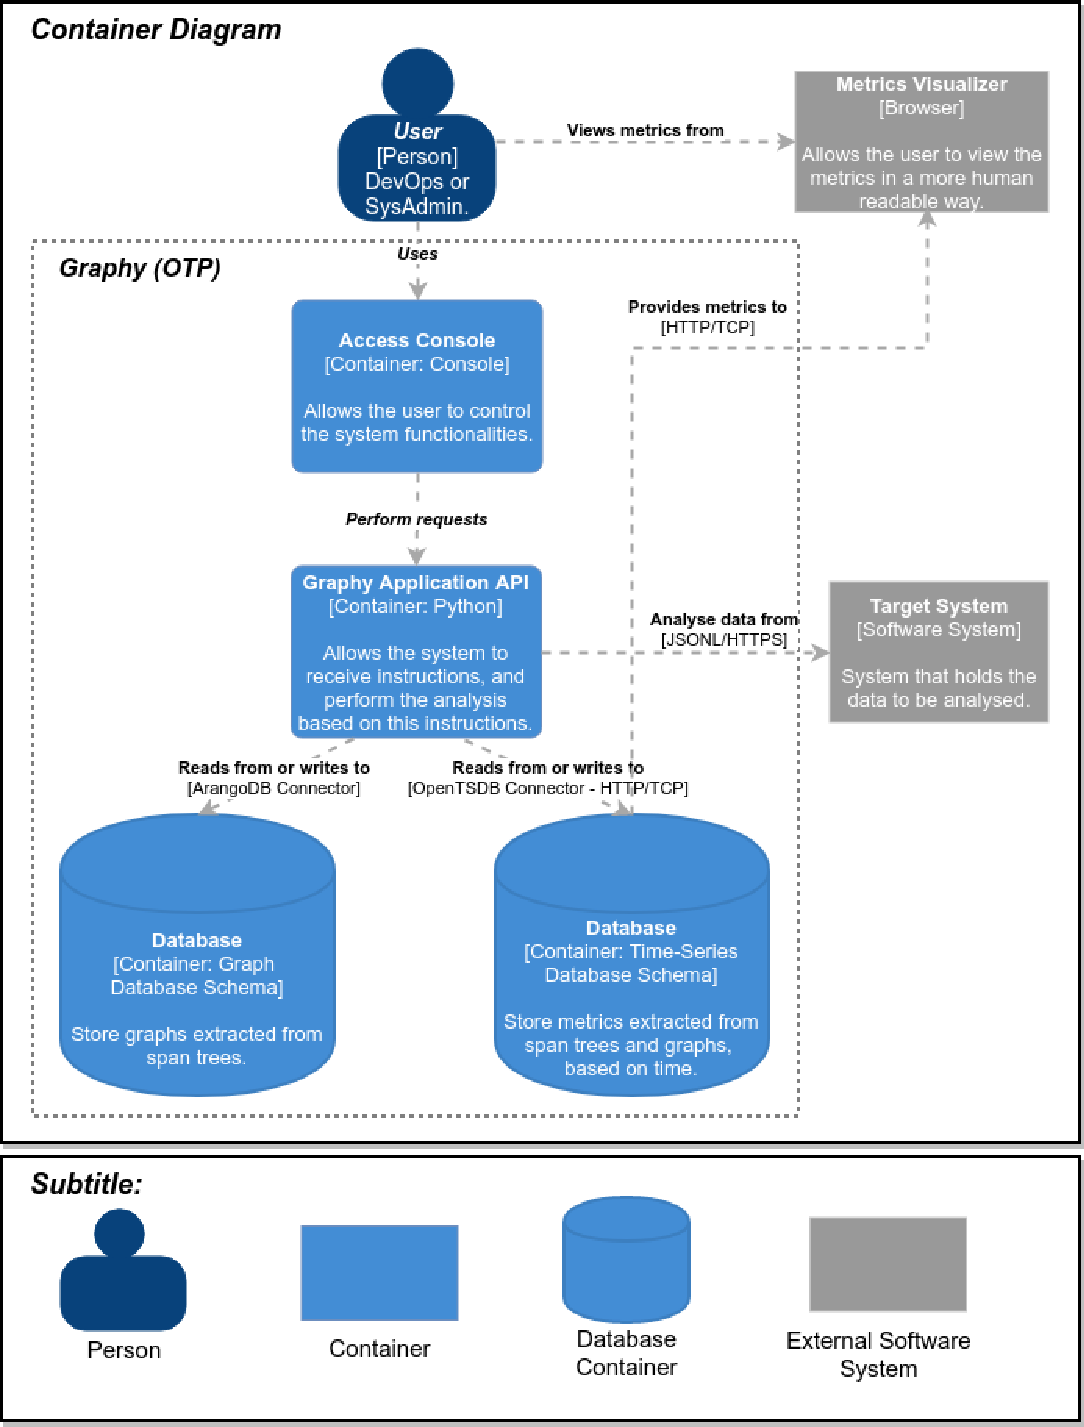
\includegraphics[width=1.00\textwidth]{images/container_diagram.pdf}
    \caption{Container diagram.}
    \label{fig:container_diagram}
\end{figure}

In this figure we can see the main containers involved in the Graphy system. The first one, from top to bottom, is the \textit{Access Console} and this container was considered as it is needed for the user to be able interact with the \textit{Graphy Application API}. The \textit{Graphy Application API} controls the entire Graphy system, that uses a communication protocol to retrieve information from the system it must analyse, and two databases to store the information resulted from the processing, a \gls{gdb} and a \gls{tsdb}.


% Component Diagram ------------------------------------------------------------------------------
\subsection{Component Diagram}
\label{subsec:component_diagram}

In this subsection, the last diagram is presented, the component diagram. This kind of diagram gives us a more deeper vision about the system, and therefore, it presents us with its main components. The figure \ref{fig:component_diagram} presents the component diagram for this solution.

\begin{figure}[!ht]
    \centering
    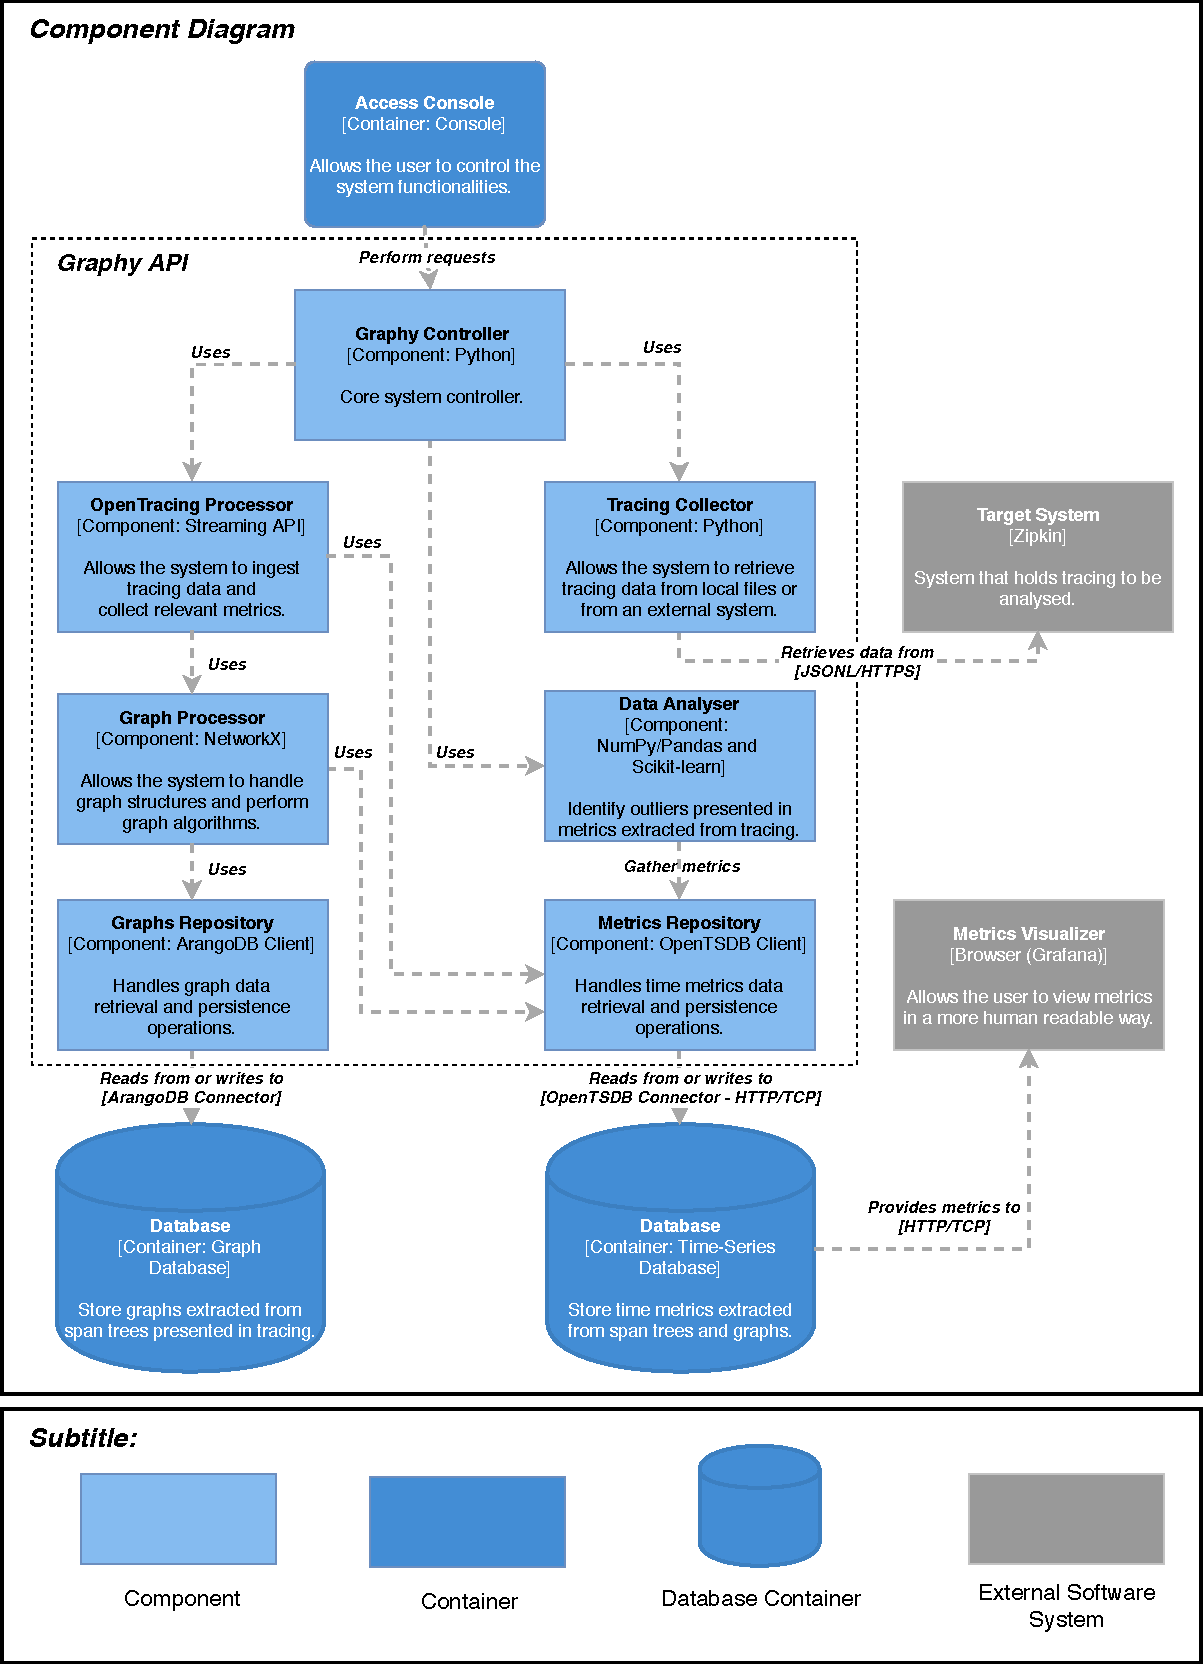
\includegraphics[width=1.00\textwidth]{images/component_diagram.pdf}
    \caption{Component diagram.}
    \label{fig:component_diagram}
\end{figure}

In this last diagram, we have a lower level of abstraction sight of the \textit{Graphy Application API} container, composed by a total of eight components. At its core we have the \textit{Graphy Controller}, that has the responsibility of controlling the remaining components involved in the system, orchestrating the actions requested by the user thought the \textit{Access Console} and performed by the whole system. In the remaining components, we have two that have greater relevance, the \textit{Graph Processor} and the \textit{Data Analyzer}. These components are responsible of processing the data converted from the Spans and Traces data, use the corresponding repository component to store or retrieve information from its database, and perform the analysis of the data. Finally we have the \textit{Testing Component}, which is responsible of test the systems algorithms, the \textit{Logging Component} which is responsible of log the relevant information and the \textit{File IO} which is responsible of handle the files involved in the system processes.

To check the architecture produced, and as said before, we will now cycle thought all the \gls{qa} and check were they are reflected in the architecture presented for this solution, and explain the trade-off involved and what were our considerations about each one.

\gls{qa}1 and \gls{qa}2 are satisfied by the simple fact that the system is able to analyse data from an external system, using a transmission protocol where data is exchanged thought HTTPS in JSONL format. As the data is only read from an exposed endpoint presented in the target system, this will not affect the normal work of the external system as this preserves its independence.

\gls{qa}3 is satisfied when we decide to use NetworkX as the technology to process our graphs. This technology does not scale horizontally, however it has a very decent performance and it's able to retrieve a certain measure of a graph with about 100.000 nodes, in near 15 seconds\cite{networkx_speed}. From 1.000.000 spans, in normal conditions, we will never be able to get a graph of this kind of size, as with our experiments, with 100.000 spans we were able to get a graph of almost 20 nodes, and with 200.000 spans we were able to get a graph of almost 30 nodes. In the end, we are considering this time and span quantity to be sure that our tool will give us good times and ease our work of performing the research and implementation of this kind of tool.

\gls{qa}4 is satisfied because we decided to use two databases that are scalable horizontally by design, the ArangoDb for a \gls{gdb} and the OpenTSDB for a \gls{tsdb}, both presented in the \ref{subsec:graph_database_tools} and \ref{subsec:time_series_database_tools} subsections respectively. In the end, this \gls{qa} can not be fully satisfied because we can not scale our system entirely, due to the fact of the technology that we chose to perform the graph processing. However, we have chosen this technology because it can perform much more graph algorithms, as we can see in the figure \ref{fig:graph_manipulation_and_performance_tools_diagram_comparison}, and this is much more relevant for our main purpose.

\gls{qa}5 is satisfied by the existence of the component \textit{Logging Component}, that allows the system to perform logging of relevant information. For the technology here, we decided to use click-log\cite{click_log_doc}, a python library used for logging purposes as it has all the main capabilities needed here to perform the logging.

\gls{qa}6, like the previous one is satisfied by the existence of a certain component, the \textit{Testing Component}, which implements all the capabilities and functionalities to perform tests and check if the systems is working correctly.

Finally, for the only technical restriction raised, we can see that it is satisfied by the usage of the OpenTSDB as our \gls{tsdb}.

With all that was presented before, we conclude that our solution satisfies all the quality attributes, business constraints and technical restrictions, and therefore, we may claim that this architecture fits our needs as a solution, taking into consideration the trade-offs involved and explained before.
%-------------------------------------------------------------------------------------------------


%-------------------------------------------------------------------------------------------------
\checkoddpage
\ifthenelse{\boolean{oddpage}}
{ % Odd page
\newpage
\blankpage}
{ % Even page
}
%-------------------------------------------------------------------------------------------------